\chapter{Materiales y métodos}
\newcommand{\ros}{\texttt{ROS}}
\section{\ros}
\ros (Robot Operative System) es un sistema operativo de código abierto basado en paso de mensajes diseñado para plataformas robóticas. Sus usos van desde el diseño de drivers, a resolver problemas complejos como la navegación autónoma.

La filosofía del sistema operativo es permitir a los desarrolladores abarcar de manera independiente los problemas que surgen al desarrollar una plataforma robótica, de modo que cada módulo pueda comunicarse con el resto, y que no haya que rediseñar un programa cuando se quiere cambiar de plataforma (y que una misma plataforma se beneficie de la implementación de distintos programas).

La versión usada para trabajar con el robot Baxter ha sido \texttt{Indigo}, ya que es la versión soportada por el robot.
\subsection{Arquitectura}
La arquitectura de \ros sigue un modelo distribuido, donde cada nodo realiza una tarea y los nodos pueden comunicarse entre sí. Esta comunicación lo hace mediante paso de mensajes.
\subsubsection{Nodos}
Los nodos son los programas que realizan las tareas, ejecutables que utilizan \ros para para comunicarse con otros nodos. Para programarlos se usan las librerías roscpp (para c++) o rospy (para Python). En el presente trabajo se utiliza la implementación en Python (por motivos de compatibilidad con la API de Baxter, así como con las librerías tensorflow y keras explicadas más adelante).

\subsubsection{Temas}
Los temas son los canales de comunicación que utilizan los nodos para comunicarse con otros nodos. Son los ``puertos'' que cada tema pone hace público para permitir la comunicación con otros nodos.

Los nodos publican y se suscriben a los temas.

\subsubsection{Mensajes}
La comunicación entre nodos se hace con el paso de mensajes. Estos son estructuras de datos que permiten a los nodos especificar y conocer la información que envían y reciben.

\subsubsection{Servicios}
Se trata de otra manera de comunicación, en la que un nodo hace una petición a otro y éste puede responder. Se diferencia de los mensajes en que el suscriptor puede responder al mensaje recibido, y su uso está enfocado a tareas aperiódicas.

\subsubsection{Parámetros}
Los parámetros son piezas de información contenidas en cada nodo que pueden ser vistas y modificadas por los nodos.

\subsubsection{Ejemplo}
Como ejemplo, se puede pensar en una cámara de vídeo que retransmite el vídeo en tiempo real. Esta cámara es un nodo (\texttt{/camera}) que publica mensajes del tipo imagen (que consiste en una matriz de nxm píxeles) al tema \texttt{/camera/image}.

Por otro lado, en un servidor estamos ejecutando un programa de detección de imágenes haciendo uso de \ros para la comunicación (nodo \texttt{/camera/server}). Este programa se suscribe al tema \texttt{/image} para recibir las imágenes que va a analizar.

Adicionalmente, la cámara tiene habilitado un servicio para reiniciar la cámara (\texttt{/camera/reset}) así como un conjunto de parámetros para filtrar las imágenes antes de publicarlas (\texttt{/color\_mode}), que permite cambiar la imagen a blanco y negro, sepia...

\subsection{\texttt{rosbag}}
\label{subsec:metodos/rosbag}
\texttt{rosbag} es una herramienta para grabar el paso de mensajes realizados sobre los temas que se le ofrecen como parámetros. Tiene la capacidad de grabar información adicional a los mensajes, como la marca temporal (momento en el que el mensaje es registrado) y de secuencia (número de mensaje en una secuencia) que cada mensaje tiene asociada. Esto es útil para sincronizar mensajes generados por otro sistema y recibidos por tcp/ip con los mensajes generados en el propio ordenador.


\section{Baxter}
% Describir temas fundamentales
\subsection{Disposición}
% en el laboratorio, cómo se ha trabajado con él
\subsection{Hardware}
% Explicar hardware y software de Baxter (procesador, JCBs, ros, interfaz de comunicación (baxter.sh))
El robot cuenta con:

\begin{itemize}
\item [2 brazos] Con 7 articulaciones (grados de libertad) cada uno y sensores que miden la posición, velocidad y torque aplicado en cada una de las articulaciones.
\item [Pantalla] En la cabeza, con la capacidad de moverse hacia los lados.
\item [3 cámaras] Una al final de cada brazo y una en la pantalla, con una resolución máxima de 1280 x 800 píxeles y una tasa de refresco de 30 cuadros por segundo. 
\item [Pinzas] Que se colocan al final de cada articulación. También se puede colocar una bomba de vacío. No interfieren con las cámaras.
\item [Sonar] Ubicado en la cabeza.
\item [Botones] Para interactuar con el robot, ubicados en los brazos, así como en el torso, a cada lado del robot.
\end{itemize}

Las articulaciones son:

\begin{itemize}
\item[s0] Rotación del hombro.
\item[s1] Traslación del brazo.
\item[e0] Rotación del brazo.
\item[e1] Traslación del antebrazo.
\item[w0] Rotación del antebrazo.
\item[w1] Traslación de la mano.
\item[w2] Rotación de la muñeca, a fin de satisfacer dicho movimiento cuando la pinza se encuentra insertada.
\end{itemize}

Dichas articulaciones se pueden observar en la figura \ref{fig:desarrollo/joints}.

\begin{figure}[]
	\centering
	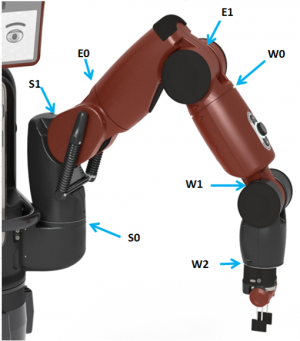
\includegraphics[width=2.5in]{imagenes/metodos/baxter_joint_names.png}
	\caption{Articulaciones del robot Baxter}
	\label{fig:desarrollo/joints}
\end{figure}

Cada brazo se puede controlar de manera independiente, pudiendo usar cada uno de ellos con un modo de control distinto. Los modos de control son los que se muestran a continuación:

\begin{enumerate}
\item Control por posición
\item Control por velocidad
\item Control por torque
\item Control por posición sin procesar (raw mode)
\end{enumerate}

Haciendo uso de la arquitectura de paso de mensajes que nos ofrece \ros, somos capaces de enviar en un tema (topic) tanto el modo de control que queremos usar como las características objetivos que queremos en el movimiento. El robot Baxter estará escuchando cada uno de los mensajes que le enviemos a los temas \texttt{/robot/limb/left/joint\_command} para el brazo izquierdo y \texttt{/robot/limb/right/joint\_command} para el brazo derecho. El tipo de mensaje que se envía es \texttt{JointCommand}, que tiene como argumentos:

\begin{itemize}
\item mode (POSITION\_MODE=1, VELOCITY\_MODE=2, TORQUE\_MODE=3, RAW\_POSITION\_MODE=4)
\item command (lista de flotantes)
\item names (lista de nombre de articulaciones)
\end{itemize}

El modo de control para cada brazo es único, mientras que la posición/velocidad/torque deseado es único para cada articulación en cada brazo.

Aparte de enviar este tipo de mensajes, podemos definir la velocidad relativa máxima que alcanzará cada articulación en el modo de control por posición publicando al tema \texttt{/robot/limb/<right/left>/set\_speed\_ratio} un valor entre 0 y 1.

El robot Baxter cuenta con una serie de limitaciones en cuanto a posiciones, velocidades y torques se refiere para cada articulación. Estas limitaciones se muestran en el cuadro \ref{tab:desarrollo/limits}.

\begin{table}[]
\centering
\caption{Límites articulaciones}
\label{tab:desarrollo/limits}
\begin{tabular}{cccccc}
Art.                    & (rad) Mín & (rad) Máx & (rad) Rango & (rad/s) Vel máx & (Nm/rad) \\ \hline
\multicolumn{1}{c|}{S0} & -1.7016   & +1.7016   & 3.4033      & 2.0             & 843      \\
\multicolumn{1}{c|}{S1} & -2.147    & +1.047    & 3.194       & 2.0             & 843      \\
\multicolumn{1}{c|}{E0} & -3.0541   & +3.0541   & 6.1083      & 2.0             & 843      \\
\multicolumn{1}{c|}{E1} & -0.05     & +2.618    & 2.67        & 2.0             & 843      \\
\multicolumn{1}{c|}{W0} & -3.059    & +3.059    & 6.117       & 4.0             & 250      \\
\multicolumn{1}{c|}{W1} & -1.5707   & +2.094    & 3.6647      & 4.0             & 250      \\
\multicolumn{1}{c|}{W2} & -3.059    & +3.059    & 6.117       & 4.0             & 250     
\end{tabular}
\end{table}
% Ratio de velocidad

\subsection{API de \ros}\label{sec:api-de-ros}
Los temas que registraremos serán:

\begin{itemize}
\item \texttt{/robot/joint\_states} Tanto la posición como la velocidad y torque de las articulaciones del brazo izquierdo.
\item \texttt{/robot/limb/left/set\_speed\_ratio} Ratio de velocidad deseada.
\item \texttt{/robot/limb/left/joint\_command} Posiciones deseadas.
\end{itemize}
subsubsec:metodos/pythonAPI\subsection{API de Python}
\label{subsubsec:metodos/pythonAPI}
La API tiene como objetivo disponer una interfaz basada en el lenguaje de programación Python para controlar y monitorizar el robot Baxter, ejecutando en su base las correspondientes instrucciones \ros. Para ello, cuenta con una serie de módulos orientados a los distintos componentes del robot (brazos, pinzas, cámara...).

Se hará uso del módulo \texttt{brazo} para realizar el movimiento del mismo. Por motivos de disposición del robot en el laboratorio, se extraerá la base de datos haciendo uso del brazo izquierdo.

Dentro de este módulo, se hará uso de las funciones \texttt{set\_joint\_position\_speed(speed)} y \texttt{move\_to\_joint\_positions(positions)}. La primera controlará la velocidad máxima relativa para cada articulación, mientras que la segunda moverá el brazo a la posición deseada. Esta función cuenta además con un intervalo de tiempo máximo para realizar el movimiento. Que el tiempo máximo se agote será indicador de que el robot no puede alcanzar la posición deseada (está colisionando consigo mismo).

Un dato a tener en cuenta es que la función \texttt{move\_to\_joint\_positions(positions)} realiza un filtro paso baja de la diferencia de posiciones (actual y deseada) en el tiempo, ofreciendo un movimiento más fluido.
\subsection{Mecanismos de control}
\label{subsec:metodos/control_baxter}
\subsubsection{Control por posición}
El control por posición consiste en alcanzar las posiciones objetivo para cada una de las articulaciones. El modo de control en el mensaje JointCommand es el 1.

La orden donde todas las articulaciones se ponen en la posición 0 corresponde con el brazo totalmente estirado y con el hombro, codo y muñeca mirando hacia abajo. Las traslaciones y rotaciones se corresponden con los de la figura \ref{fig:desarrollo/joint_map}.

\begin{figure}[]
	\centering
	\begin{subfigure}[b]{0.4\textwidth}
		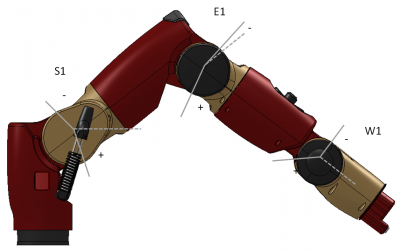
\includegraphics[width=\textwidth]{imagenes/metodos/baxter_range_motion1.png}
		\caption{Límites traslación}
		\label{fig:desarrollo/limits1}
	\end{subfigure}
	\begin{subfigure}[b]{0.4\textwidth}
		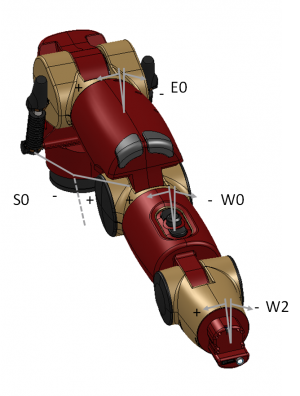
\includegraphics[width=\textwidth]{imagenes/metodos/baxter_range_motion2.png}
		\caption{Límites rotación}
		\label{fig:desarrollo/limits2}
	\end{subfigure}
	\caption{Límites articulaciones}
	\label{fig:desarrollo/limits}
\end{figure}

Dada la naturaleza del robot Baxter, en este modo de operación se aplican unos filtros antes de aplicar la orden de posición, a fin de evitar accidentes y otorgar una experiencia de movimiento más fluida y segura. Los filtro son los que se muestran en la figura \ref{fig:desarrollo/position_filters}.

\begin{figure}[]
	\centering
	\begin{subfigure}[b]{0.24\textwidth}
		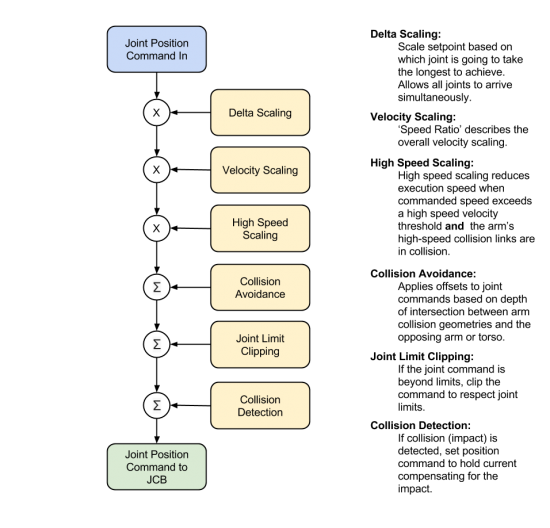
\includegraphics[trim=0 0 235 0, clip, width=\textwidth]{imagenes/metodos/baxter_position_filters.png}
		\caption{Control por posición}
		\label{fig:desarrollo/position_filters}
	\end{subfigure}
	\begin{subfigure}[b]{0.24\textwidth}
		\centering
		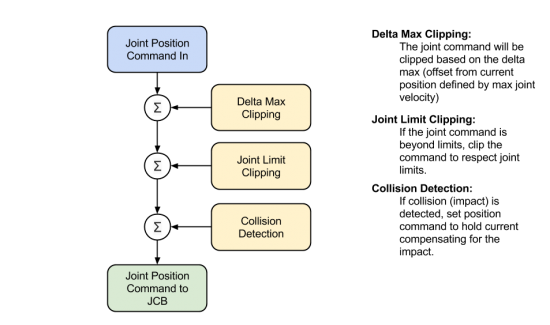
\includegraphics[trim=0 0 230 0, clip, width=\textwidth]{imagenes/metodos/baxter_position_raw_filters.png}
		\caption{Control por posición sin procesar}
		\label{fig:desarrollo/raw_filters}
	\end{subfigure}
	\begin{subfigure}[b]{0.24\textwidth}
		\centering
		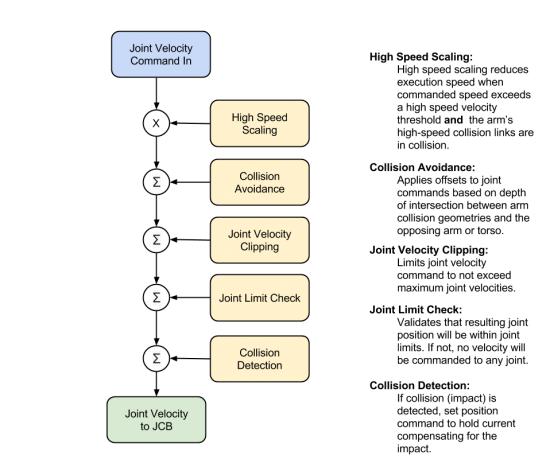
\includegraphics[trim=0 0 235 0, clip, width=\textwidth]{imagenes/metodos/baxter_velocity_filters.png}
		\caption{Control por velocidad}
		\label{fig:desarrollo/vel_filters}
	\end{subfigure}
	\begin{subfigure}[b]{0.24\textwidth}
		\centering
		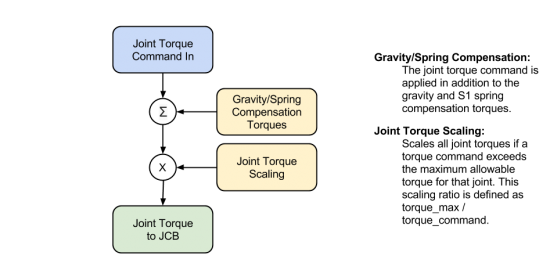
\includegraphics[trim=0 0 230 0, clip, width=\textwidth]{imagenes/metodos/baxter_torque_filters.png}
		\caption{Control por torque}
		\label{fig:desarrollo/torque_filters}
	\end{subfigure}
	\caption{Filtros aplicados}
\end{figure}

\begin{enumerate}
\item [Escalado delta] Consiste en escalar las posiciones objetivo en el recorrido para conseguir que todas las articulaciones lleguen al punto deseado a la vez.
\item [Escalado de velocidad] Se escala la velocidad de cada articulación en función del 'ratio de velocidad'.
\item [Escalado de alta velocidad] Para evitar colisiones entre los dos brazos moviéndose el uno en la dirección del otro, se escala la velocidad y recalcula la posición cuando ésta supera un umbral.
\item [Prevención de colisiones] Gracias a un modelo interno del robot, se limitan las posiciones de las articulaciones tales que provocarían un choque con el propio robot.
\item [Recorte de posiciones] Si las posiciones superan los límites de la articulación, estas se recortan al límite permitido.
\item [Detección de colisión] Si se detecta una colisión (con un objeto externo al robot), mantiene la última posición antes de la colisión.
\end{enumerate}

Como se puede observar, Baxter aplica unos filtros para evitar y detectar colisiones. Esta tarea se realiza de tres maneras:

\begin{itemize}
\item [Prevención] El robot ejecuta una simulación interna, donde las articulaciones y el cuerpo cuentan con unas regiones de seguridad que, al tocarse, limitan el movimiento del robot.
\item [Detección de colisión] Esto se realiza de dos maneras
\begin{enumerate}
\item [Impacto] Cuando el torque de cualquier articulación cambia bruscamente, se considera que ha habido una colisión.
\item [Retención] Cuando el torque aplicado aumenta pero la articulación no se mueve, se considera que está colisionando con un objeto inmóvil.
\end{enumerate} 
\item [Escalado de alta velocidad] Cuando la velocidad del brazo supera los 0.2 m/s, las regiones de seguridad que el robot simula internamente aumentan. Cuando se tocan estas regiones, la velocidad se escala y la posición se recalcula.
\end{itemize}

\subsubsection{Control por posición sin procesar}
Este modo de control, al igual que el anterior, tiene como objetivo alcanzar la posición deseada para cada articulación. Se diferencia en los filtros que aplica (figura \ref{fig:desarrollo/raw_filters}).

\begin{enumerate}
\item [Recorte de delta máximo] Recorta la posición siguiente (en el intervalo de actuación de cada articulación) a la máxima posición alcanzable a la velocidad máxima dada por la 'ratio de velocidad'.
\item [Recorte de posiciones] Al igual que en el modo de control anterior, si las posiciones superan los límites de la articulación, estas se recortan al límite permitido.
\item [Detección de colisión] Cumple la misma función que en el modo de control por posición.
\end{enumerate}

Como se puede observar, este es un modo de control más avanzado, ya que no tiene en cuenta las colisiones consigo mismo, y ofrece un movimiento más brusco al no llegar todas las articulaciones al punto destino a la vez.

El modo de control en el mensaje JointCommand es el 4.

\subsubsection{Control por velocidad}
En este modo de control, lo que se busca es adquirir la velocidad objetivo para cada articulación. El modo de control en el mensaje JointCommand es el 2. Al igual que en los modos anteriores, se aplican una serie de filtros (figura \ref{fig:desarrollo/vel_filters}).

\begin{enumerate}
\item [Escalado de alta velocidad] Como en el control por posición.
\item [Prevención de colisiones] Como en el control por posición.
\item [Recorte de velocidades] Se limitan las velocidades para cada articulación para que no excedan el máximo permitido.
\item [Comprobación de límites] Se comprueban los límites de las articulaciones. Si se exceden, se detiene el movimiento.
\item [Detección de colisión] Igual que en el control por posición.
\end{enumerate}

El dejar de enviar velocidades si se exceden los límites de las articulaciones es una medida de seguridad que exige al programador tener el control sobre las posiciones que puede alcanzar el brazo.

\subsubsection{Control por torque}
El control por torque consiste en el modo de más bajo nivel que se puede controlar el robot Baxter. Los torques que enviemos serán aplicados por los controladores, haciendo uso solamente de los siguientes filtros (figura \ref{fig:desarrollo/torque_filters}):

\begin{enumerate}
\item [Compensación] Los torques se suman a los necesarios para mantener la gravedad 0 y el muelle ubicado en la articulación s1 (traslación del hombro).
\item [Escalado de torque] Si un torque excede el torque máximo para esa articulación, escala los torques de todas las articulaciones por el factor de exceso de esa articulación (torque\_max/torque).
\end{enumerate}

La compensación de la gravedad se puede desactivar mandando un mensaje vacío al tema \texttt{/robot/limb/right/suppress\_gravity\_compensation} para el brazo derecho, o \texttt{/robot/limb/left/suppress\_gravity\_compensation} para el brazo izquierdo.

De esta manera, un torque aplicado de 0 en todas las articulaciones, mantendrá el brazo en un estado de gravedad 0 si la compensación esta activa. De no estarlo, el brazo caerá en peso muerto.

\subsection{Simulador}

\section{Redes Neuronales}
Una red neuronal artificial es un conjunto de algoritmos de aprendizaje automático capaces de extraer modelos a partir de un conjunto de datos de aprendizaje. De esta manera, estos sistemas son capaces de emular la fuente generadora de datos y producir salidas coherentes a partir de entradas no vistas con anterioridad.
\subsection{Topología}
En función de la topología de la red, se contemplan dos tipos fundamentales:
\subsubsection{Redes hacia adelante}
Las conexiones entre las neuronas es de un solo sentido, de modo que no se forman bucles entre ninguna de las neuronas (figura \ref{fig:metodos/feedforward}).

\begin{figure}
	\centering
	\begin{neuralnetwork}[height=4.7]
		\newcommand{\nodetextclear}[2]{}
		\newcommand{\nodetextx}[2]{$x_#2$}
		\newcommand{\nodetexty}[2]{$y_#2$}
		\inputlayer[count=4, bias=false, title=Capa de\\entrada, text=\nodetextx]
		\hiddenlayer[count=5, bias=false, title=Capa\\oculta, text=\nodetextclear] \linklayers
		\outputlayer[count=3, title=Capa de\\salida, text=\nodetexty] \linklayers
	\end{neuralnetwork}
	\caption{Red neuronal de propagación hacia adelante}
	\label{fig:metodos/feedforward}
\end{figure}
\paragraph{Propagación hacia atrás de errores}
\subsubsection{Redes realimentadas}
\paragraph{Propagación hacia atrás de errores en el tiempo}
\subsubsection{Aprendizaje profundo}
\subsection{Herramientas}
\subsubsection{Tensorflow}
\subsubsection{Keras}
\section{Controladores}
\subsection{Error distal}
\subsection{Control realimentado}
\subsection{Control Anticipativo}